\section{Affine algebraische Gruppen}
\label{sec:para1}
\subsection{Affine algebraische Varietät}
\label{sub:abschnitt_1.1}

\begin{defn}[Affine algebraische Menge]
	Sei $k = \overline{k}$ ein algebraisch abgeschlossener Körper,\marginnote{27.10.} $\aff_k^n := \{ (x_1,\dots,x_n) : x_i \in k\}$ sowie $I = (f_1,\dots,f_r) \subseteq k[x_1,\dots,x_n]$ ein Ideal. Wir bezeichnen
	\[ V(I) = \{x \in \aff_k^n : f(x) = 0 \text{ für } f \in I\} \]
	als \Index{affine algebraische Menge}.
\end{defn}

\begin{bsp}
	\begin{enumerate}[a)]
		\item Sei $f = \sum_{i=1}^{n} a_ix_i + c$ eine allgemeine lineare Gleichung, o.E. $a_1 \neq 0$. Dann ist $V(f)$ eine Hyperebene isomorph zu $\aff_k^{n-1}$. \\
		Im Fall $f=0$ ist $V(0) = \aff^n$ und im Fall $f = c \neq 0$ ist $V(c) = \emptyset$.
		\item Wir betrachten Quadriken. Sei $f$ quadratisch von der Gestalt
		\[ f = \underbrace{\sum_{1\leq i \leq j \leq n} a_{ij} x_i x_j}_{=: q \neq 0} + \underbrace{\sum_{x=1}^{n} b_i x_i}_{=: l} + c \]
		Idee: $f$ auf einfachere Gestalt bringen, z.B. mit $q$ in Diagonalform:
		\[ f = \sum_{i=1}^{n} a_i x_i + \sum_{i=1}^{n} b_i x_i + c \]
		mit $a_i \in \{0,1\}$ nach Skalierung. Koordinaten vertauschen:
		\[ f = \sum_{i=1}^{m} x_i^2 + \sum_{i=1}^{n} b_i x_i + c, \quad 1 \leq m \leq n \]
		Quadratische Ergänzung:
		\[ f = \sum_{i=1}^{m} x_i^2 + \sum_{i=m+1}^{n} b_i x_i + c \]
		Nun Beispiel a) anwenden:
		\[ f = \sum_{i=1}^{n} x_i^2 + c, c \in \{0,1\} \qquad \qquad \qquad f = \sum_{i=1}^{m} x_i^2 + x_n, m < n \]
		
		$n=2$:\todo{Das Wort "Skizze" sollte etwas höher stehen.} \\
		\begin{tabular}{rccc}
			& $x^2 + y^2 = 0$ & $x^2+y^2 = 1$ & $x^2 = y$ \\ 
			andere Varianten: & $x^2-y^2 = 0$ & $x^2-y^2=1$ &  \\ 
			Skizze: & 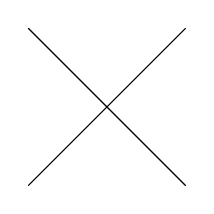
\begin{tikzpicture}
				\draw (-1,-1) -- (1,1);
				\draw (-1,1) -- (1,-1);
			\end{tikzpicture} & 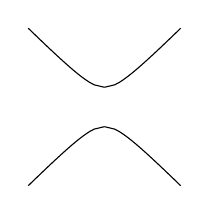
\begin{tikzpicture}[scale=0.5,rotate=90]
				\draw plot[domain=0.5:2] (\x,{(\x*\x-0.25)^(1/2)});
				\draw plot[domain=0.5:2] (\x,{-(\x*\x-0.25)^(1/2)});
				\draw plot[domain=-2:-0.5] (\x,{(\x*\x-0.25)^(1/2)});
				\draw plot[domain=-2:-0.5] (\x,{-(\x*\x-0.25)^(1/2)});
			\end{tikzpicture} & \begin{tikzpicture}[scale=0.5]
				\draw plot[domain=-2:2] (\x,{\x*\x});
			\end{tikzpicture} \\ 
			& zwei sich schneidende Geraden & Kreis (reell) bzw. Hyperbel (komplex) & Parabel
		\end{tabular} 
		
		$n = 3$: \todo{Hier fehlen drei Grafiken.}
		\[\begin{array}{ccc}
			x^2+y^2-z^2 = 0 & x^2+y^2-z^2=1 & x^2+y^2=z \\ 
			&  &   
		\end{array} \]
		Sei $f = x^2+y^2+z^2$ und $g = x^2+y^2+z$. \\
		\begin{equation}
		\begin{aligned}
			f(\vec{x_0} + t\vec{x}) &= (x_0 + tx)^2 + (y_0 + ty)^2 + (z_0 + tz)^2 \\
			&= 2t(x_0x+y_0y+z_0z) + x_0^2 + y_0^2 + z_0^2 + \text{ quad. Term} \\
			g(\vec{x_0}+t\vec{x}) &= 2t(x_0x+y_0y)+tz+x_0^2+y_0^2+ \text{ quad. Term}
		\end{aligned}
		\end{equation}
		\[ T_{(x_0,y_0,z_0)}Q = \{ (x,y,z) : \sprod{(x_0,y_0,z_0),(x,y,z)} = 0\} \qquad T_{(x_0,y_0,z_0)}Q = \{(x,y,z) : z = -2(x_0x + y_0y)\}\]
		\[ \dim T_{x_0}Q = \begin{cases}
			2 & (x_0,y_0,z_0) \neq 0 \\
			3 & (x_0,y_0,z_0) \neq 0
		\end{cases} \hspace{5cm}  \dim T_{x_0}Q = 2 \]
	\end{enumerate}
\end{bsp}
	
\subsection{Affine algebraische Varietät (ja, der Abschnitt hieß auch so!)}
\label{sub:abschnitt_1.2}
	$Z(I) := V(I)$		\marginnote{Bezeichnungen ändern sich aus irgendeinem nicht ersichtlichen Grund!} \\
	$a \subseteq S := k[x_1,\dots,x_n] \ni f_1, \dots, f_r, \quad I = (f_1,\dots, f_r)$ \\
	$T \subseteq S$ beliebige Teilmenge \\
	$Z(T) = \{p \in \aff^n : f(p) = 0 \text{ für alle } f \in T\}$ Nullstellenmenge
	
\begin{defn}
	Eine Teilmenge $Y \subseteq \aff^n$ heißt genau dann \bet{algebraisch}, falls $Y = Z(T)$ für eine Teilmenge $T \subseteq S$. \index{algebraische Teilmenge}
\end{defn}

\begin{satz}
	\begin{enumerate}[1)]
		\item $Z(T_1) \cup Z(T_2) = Z(T_1 \cdot T_2)$,
		\item $Z \enbrace*{\bigcup\limits_{i \in I} T_i} = \bigcap\limits_{i \in I} Z(T_i)$,
	\end{enumerate}
	d.h. die abgeschlossenen Teilmengen bilden eine Topologie.
\end{satz}

\begin{bsp}
	\begin{itemize}
		\item In $\aff^1$ sind die abgeschlossenen Teilmengen genau die endlichen Mengen und $\aff^1$.
		\item In $\aff^2$ sind die abgeschlossenen Teilmengen genau die endlichen Mengen, $\aff^2$ sowie endliche Vereinigungen $V(f_1) \cup \dots \cup V(f_r)$ (ohne Beweis)
		\item Die von den abgeschlossenen Mengen erzeugte Topologie ist nicht $T_2$: $p \in \aff^1$, $U \ni p$ offen, $Q \in \aff^1 \setminus U$, $V \supset Q$ offen $\Rightarrow U \cap V \neq \emptyset$.
	\end{itemize}
\end{bsp}
	
\begin{defn}[Irreduzibler topologischer Raum]
	Ein topologischer Raum $Y \neq \emptyset$ heißt \Index{irreduzibel}, falls gilt:
	\[Y = Y_1 \cup Y_2 \text{ mit } Y_1,Y_2 \text{ abgeschlossen} \quad \Rightarrow \quad Y_1 \subseteq Y_2 \text{ oder } Y_2 \subseteq Y_1 \]
\end{defn}

\begin{bsp}
	\begin{itemize}
		\item $\aff^1$ ist irreduzibel (später: $\aff^n$ ist irreduzibel)
		\item Folgende Quadriken sind irreduzibel: $f = X_1^2 + \dots + X_{n-1}^2 + X_n$ für $n \geq 1$, $f = X_1^2+ \dots + x_n^2 + 1$ für $n \geq 2$, $f = \sum_{i=1}^{n \geq 3} x_i^2$
		\item $V(x(x-1)) = \{ (0),(1) \}$ ist nicht irreduzibel.
		\item $x_1^2 + 1$, $x_1^2+x_2^2 = 0$ sind nicht irreduzibel
		\item $Y \subseteq X$ irreduzibel (mit induzierter Topologie) $\Rightarrow \overline{Y}$ irreduzibel.
	\end{itemize}
\end{bsp}

\begin{defn}[affine algebraische Varietät]
	Sei $\mathfrak{a}$ ein Ideal. $Z(\mathfrak{a})$ heißt \Index{affine algebraische Varietät}, falls $Z(\mathfrak{a})$ irreduzibel ist.
\end{defn}

\subsection{Ideale}	\label{sub_1.3}
	Sei $Y \subseteq \aff^n$\marginnote{30.10.} Teilmenge und $I(Y) = \{f \in S = k[x_1,\dots,x_n] : f(x) = 0 \text{ für alle } y \in Y\}$ das Verschwindungsideal von $Y$. Sei $T \subseteq S$ und $Z(T)$ die Nullstellenmenge von $T$.
	
\begin{satz}
	\begin{enumerate}[a)]
		\item $T_1 \subseteq T_2 \Rightarrow Z(T_1) \supseteq Z(T_2)$
		\item $Y_1 \subseteq Y_2 \subseteq \aff^n \Rightarrow I(Y_1) \supseteq I(Y_2)$
		\item $Y_1,Y_2 \subseteq \aff^n \Rightarrow I(Y_1 \cup Y_2) = I(Y_1) \cap I(Y_2)$
		\item $\mathfrak{a} \subseteq S$ Ideal $\Rightarrow I(Z(\mathfrak{a})) = \sqrt{\mathfrak{a}} := \{f \in S : f^m \in \mathfrak{a} \text{ für ein } m\}$ (\Index{Radikal} von $\mathfrak{a}$) 
		\item $Y \subseteq \aff^n, Z(I(Y)) = \overline{Y}$ Abschluss von $Y$ in Zariski-Topologie.
	\end{enumerate}
\end{satz}

\minisec{Beweis}
	Nur d) mit Hilberts Nullstellensatz: \\
	$f$ verschwindet auf $Y \Leftrightarrow f^m$ verschwindet auf $Y$. $f \in I(Z(\mathfrak{a})) \xLongrightarrow{\text{Hilbert}} f^m \in \mathfrak{a}$. \qed

\begin{satz}
	\[ \begin{array}{rcl}
	\{\text{abgeschlossene Teilmengen in } \aff^n\} & \xlongleftrightarrow{1:1} & \{\text{radikale in } \mathfrak{a} \text{ in } S, \mathfrak{a} = \sqrt{\mathfrak{a}}\} \\ 
	 \rotatebox{90}{$\subseteq$} \qquad \phantom{a} &  & \qquad \rotatebox{90}{$\subseteq$} \\ 
	\{\text{irreduzible Teilmengen}\} & \xlongleftrightarrow{1:1} & \{\text{Primideale in } S\} \marginnote{$p$ PI $\Rightarrow \sqrt{p} = p$}
	\end{array}  \]
\end{satz}

\minisec{Bemerkung}
	$p$ ist genau dann ein Primideal, wenn gilt:
	\[ fg \in p \Rightarrow f \in p \text{ oder } g \in p\]
	Damit gilt: $f^n \in p \Rightarrow f \in p$ oder $f^{n-1} \in p \Rightarrow \dots \Rightarrow f \in p$ \\
	$(X^2) \subseteq k[X] \rightarrow \sqrt{(X^2)} = (X)$.
	
\minisec{Bemerkung}
	Ist $f \in S$ irreduzibel, dann heißt $Z(f)$ \Index{Hyperfläche} in $\aff^n$.
	
\minisec{Beispiel}
	$Q \subseteq \aff^n$ Quadrik ist eine Hyperfläche. \\
	maximale Ideale: $(x_1-\lambda_1, \dots, x_n - \lambda_n) = \maxid = \maxid_{\underline{\lambda}}$ mit $\underline{\lambda} = (\lambda_1,\dots,\lambda_n) \in \aff^n$ \\
	$Z(\maxid) = \{ \underline{\lambda} \}$ Einpunktmenge ist als minimale abgeschlossene nicht-lineare Teilmenge irreduzibel.
	
	$k = \RR \neq \overline{k}, Z(X^2+Y^2+1) = \emptyset \Rightarrow$ Theorem ist falsch, da $X^2+Y^2+1$ irreduzibel.  \\
	Trick: $f_1,\dots,f_r \in k[\underline{x}]$, $V(f_1,\dots,f_r) = \{ (x_1,\dots,x_n) : \aff_{\overline{k}}^n : f_i(\underline{x}) = 0 \text{ für alle } i\}$
	
Sei $Y = Z(\mathfrak{a})$ eine algebraische Teilmenge in $\aff^n$, dann definieren wir den \Index{Koordinatenring} von $Y$:
\[ A(Y) := "k[Y]" = S/\sqrt{\mathfrak{a}} \]
Ist $Y$ irreduzibel oder eine algebraische Varietät, dann ist $A(Y)$ ein Integritätsbereich. Setze $K(Y) := \Quot(A(Y))$.

Sei $\overline{f} \in A(Y)$, dann können wir $\overline{f}$ als Funktion $Y \rightarrow k$ auffassen, denn: \\
Sei $f \in S, f\colon \aff^n \rightarrow k, f \big|_Y \colon Y \rightarrow k$. Wir wollen $f \big|_Y \in A(Y)$. \\
Sei $f' \in S$ mit $f - f' \in \mathfrak{a}$, d.h. $\overline{f} = \overline{f'}$ in $A(Y) = S/\mathfrak{a}$ ($\mathfrak{a} = \sqrt{\mathfrak{a}}$, da irreduzibel) \\
$\Rightarrow f \big|_Y = f'\big|_Y$, d.h. $\overline{f} = \overline{f'} \colon Y \rightarrow k$ Funktion, d.h. Elemente von $A(Y)$ sind Funktionen auf $Y$ mit Werten in $k$.

\begin{defn}[Lokalisierung]
	Sei $A = A(Y)$ endlich erzeugter Integritätsring über $k = \overline{k}$, z.B. $A = k[x_1,\dots,x_n]/I$ mit $I$ Primideal. \begin{enumerate}[1)]
		\item $A_{(0)} = \Quot(A), \Quot(A(Y)) =: K(Y)$
		\item $A_p = \penbrace*{\frac{f}{g} \in \Quot(A) : g \notin p}$ \qquad \Index{Lokalisierung} nach einem Primideal \\
		$A_p$ und $\Quot(A)$ sind im Allgemeinen nicht endlich erzeugte Ringe
		\item $A_f = \penbrace*{ \frac{g}{f^n} : g \in A, n \geq 0}, f \in A$ \qquad \Index{Lokalisierung} nach einem Element \marginnote{$A_f \neq A_{(f)}$ !}
	\end{enumerate}
\end{defn}

\begin{defn}[Lokaler Ring]
	Ein Ring $A$ heißt \bet{lokal}, falls $A$ ein eindeutiges maximales Ideal besitzt. \index{lokaler Ring}
\end{defn}

\minisec{Beispiele}
	\begin{itemize}
		\item Sei $K$ ein Körper, dann ist $\setnull$ das einzige echte Ideal und maximal.
		\item $pA_p = (p) \subseteq A_p$ ist maximales Ideal
		\item $k[x]_{(x-1)} = \penbrace*{ \frac{f}{g} : g \notin (x- \lambda)} = \penbrace*{\frac{f}{g} : g(\lambda) \neq 0}$ \\
		$(x-\lambda) = (x - \lambda) k[x]_{(x-\lambda)} = \penbrace*{ \frac{f}{g} : f(\lambda) = 0, g(\lambda) \neq 0} \subseteq k[x]_{(x-\lambda)}$ Hauptideal \\
		Einheiten in $k[x]_{(x-\lambda)} = \penbrace*{ \frac{f}{g} : f(\lambda) \neq 0, g(\lambda) \neq 0} = k[x]_{(x-\lambda)} \setminus (x-\lambda)$
		\item $\ZZ_3 = \penbrace*{ \frac{a}{3^i} : a\in \ZZ, i \in \ZZ_0}$ \\
		$\ZZ_3^\times = \{ \pm 3^i : i \in \ZZ\}$
		\item $k[x]_{x-\lambda} = \penbrace*{ \frac{g}{(x-\lambda)^i} : g \in k[x]}$ \\
		$k[x]_{x - \lambda}^\times = \{a(x-\lambda)^i : i \in \ZZ, a \in k^\times\}$		
	\end{itemize}
	
\begin{defn}[noetherscher topologischer Raum]
	Ein topologischer Raum $X$ heißt \Index{noethersch}, falls jede absteigende Kette abgeschlossener Teilmengen $Y_1 \supseteq Y_2 \supseteq Y_3 \supseteq \dots$ stationär wird, d.h. es gibt ein $r \in \NN$, sodass $Y_r = Y_i$ für alle $i > r$.
\end{defn}

\minisec{Beispiel}
	$\aff^n$ ist ein noetherscher topologischer Raum, weil $S$ ein noetherscher Ring ist. Sei $Y_1 \supseteq Y_2 \supseteq \supseteq \dots$ eine Kette von algebraisch abgeschlossenen Teilmengen, dann ist $I(Y_1) \subseteq I(Y_2) \subseteq \dots$ aufsteigende Kette von Idealen in $S = k[\underline{x}]$ und wird stationär, d.h. $I(Y_r) = I(Y_i)$ für $i \geq r \Rightarrow Y_r = Z(I(Y_i)) = Y_i = Z(I(Y_i))$ für alle $i \geq r$.
	
\begin{defn}[Dimension (topologischer Raum, algebraische Varietät)]
	Ein topologischer Raum $X$ hat die Dimension
	\[ \dim(X) = \sup \{r \in \ZZ_{\geq 0} : \text{ es ex. Kette } Z_0 \subsetneq Z_1 \subsetneq \dots \subsetneq Z_r \text{ von irreduziblen abgeschlossenen Teilmengen } Z_i \} \]
	Die Dimension einer algebraischen Varietät $X$ entspricht der Dimension von $X$ als topologischer Raum bzgl. der Zariski-Topologie.
\end{defn}	
	
\begin{satz}
	In einem noetherschen topologischen Raum $X$ ist jede abgeschlossene Teilmenge $Y$ eine endliche Vereinigung $Y = Y_1 \cup \dots \cup Y_r$ von irreduziblen abgeschlossenen Teilmengen $Y_i$. Fordern wir zusätzlich $Y_i \nsubseteq Y_j$ für $i \neq j$, dann ist die Zerlegung eindeutig bis auf Umordnung.
\end{satz}

\minisec{Beweis}
	Existenz: Sei $\mathcal{S} := \{Y \subseteq X \text{ abgeschlossen } : Y \text{ besitzt keine solche Zerlegung} \}$. \\
	$X$ noetherscher topologischer Raum $\Rightarrow \mathcal{S}$ hat minimales Element oder ist leer. Sei $Y \in \mathcal{S}$ minimal, dann ist $Y$ nicht irreduzibel, also $Y = Y' \cup Y''$ mit $Y' \nsupseteq Y'' \nsupseteq Y'$ algebraische Teilmengen. Wegen Minimalität ist $Y', Y'' \notin \mathcal{S}$. \\
	$\Rightarrow Y' = Y_1' \cup \dots \cup Y_r', Y'' = Y_1'' \cup \dots \cup Y_s''$ 
	$\Rightarrow Y = Y_1' \cup \dots \cup Y_r' \cup Y_1'' \cup \dots \cup Y_r''$ \\
	
	Eindeutigkeit: Sei $Y = Y_1' \cup \dots \cup Y_s' = Y_1 \cup \dots \cup Y_r$ zwei Zerlegungen. Dann ist $Y_1' \subseteq Y = \bigcup_{i=1}^r Y_i$ \\
	$\Rightarrow Y_1' = \bigcup_{i=1}^r (Y_1' \cap Y_i)$ irreduzibel $\Rightarrow Y_1' \subseteq Y_i$, o.B.d.A. $i=1$. $Y_1 \subseteq Y = \bigcup_{j=1}^s Y_j' \Rightarrow \dots \Rightarrow Y_1 \subseteq Y_j' \Rightarrow j=1.$ \\
	$z = \overline{(Y \setminus Y_1)} = Y_2 \cup \dots \cup Y_r = Y_2' \cup \dots \cup Y_s' \xRightarrow{\text{Ind.}} r=s, Y_i = Y_i'$ \qed